\section{Implementation}
    In the following chapter the implementation details of the application will be described. It covers most of the application code and the design decisions around it, as well as some more theoretical content relating to the chosen implementation language \textit{Rust}. It finishes off with a closer look at some of the notable issues that arose during development, as well as various accomplishments that the reader would not have otherwise thought about.

    \subsection{Rust}
        The chosen implementation language for the project is \textit{Rust}, more details on the decision-making surrounding this choice can be found in \autoref{sec:language}.
        
        Rust is a very low-level programming language, similar in style and functionality to C, however it is built with a "memory safety first" approach. What this means in practice is that the compiler's static analysis detects most, if not all, ways of unsafe memory access and manipulation patterns, and fails the compilation if such a mistake is detected. It is possible to override these checks by using \textit{unsafe} code blocks, this is however mostly only used in \textit{FFI}\footnote{Foreign Function Interface - used for interaction with libraries written in other languages}, as idiomatic \textit{Rust} can, and should, be written with fully memory-safe code.
        
        The advanced static analysis of the compiler is known as \textit{zero-cost abstractions}. This name is derived from the fact that most of the features of \textit{Rust} come at absolutely zero overhead, because they are bound to the compilation phase - generally, if there is a problem with the code, it will fail to compile. This is in stark contrast with most other programming languages, which often encounter possibly hard to debug run-time errors. With \textit{Rust}, encountering a run-time error is very rare if the code is idiomatic. It is still possible for the program to crash, this is however usually caused either by a system error (e.g. out of memory), or by a \textit{thread panic} - a crash manually called by the programmer, or automatically generated if a failure case is left unhandled (which is once again a conscious choice of the programmer). In addition to memory safety, \textit{Rust} contains other convenience features which, once again, usually come with zero or minimal overhead. One of these are what other languages call \textit{optional types}. In \textit{Rust}, there are two kinds of \textit{optional types}: an \textit{Option} and a \textit{Result}. These can either depict a result of an operation that returns \textit{something} or \textit{nothing}, or a choice between \textit{something} and an \textit{error}. Considering the language doesn't have exceptions, these \textit{optional types} make it a breeze when an operation should return a value, however also has a chance of failure. The \textit{Option} type is a special kind of \textit{Result} that doesn't return an \textit{error} but a \textit{nothing} - this becomes very useful when an operation doesn't have to return a value; normally it would have to allocate an empty structure to return (e.g. array or hashmap), with the \textit{Option} type it can return a more simple \textit{nothing} value.
        
        The learning curve of the language isn't very steep, unless one wants to delve into advanced topics. If there's familiarity with a strongly-typed programming language such as C\# or Java, covering the basics of \textit{Rust} will take minimal time (even less if one is familiar with low level languages such as C or C++). The hardest part about learning the language is probably trying to write idiomatic code, as it will require forgetting standard practices from other languages for which \textit{Rust} provides a better, more idiomatic way (e.g. correct usage of the \textit{optional types}).
        
        I have personally started learning \textit{Rust} about half a year before fully starting the development of the project. The reasoning behind such an early start was that I would like to acquire at least semi-intermediate knowledge of the language and its best practices before using it for such a large project as this one. The most helpful resources were the "official \textit{Rust} book" \cite{rust-book}, and because I'm a large fan of reading actual documentation (which seems to be rare these days\footnote{Personal opinion formed by observation of my peers}) I also enjoyed the official library reference. In addition to these resources I read countless articles, blog posts, and other forms of online communications while either trying to solve a problem, or just while generally catching up with the news (\textit{Rust} is very popular on numerous online forums related to programming or technology).
        
    \subsection{Threading model}\label{sec:threads}
        \textsc{Liebert} utilizes a fairly complex threading model. This comes from the fact that currently there is no asynchronous I/O in \textit{Rust}. As most functions of the application are I/O-bound, be it network or the local filesystem, they require a separate thread to be spawned as to not impede the functionality of the rest of the application.
        
        Due to memory safety and parallelism being a cornerstone of \textit{Rust}, creation and management of threads is extremely simple. This meant that the usage of threads extended beyond I/O bound tasks, and is used to divide the application into independently running "modules". Utilizing this approach also means that data can be easily processed or reformatted when being exchanged between different "modules" (read more in \autoref{sec:data-flow}). An introspection into \textsc{Liebert}'s threads as seen by the Linux utility \textit{htop} can be seen in \autoref{fig:thread-list}. Note that each thread is also appropriately named, so that they can be easily analyzed.
    
            \begin{figure}[!htb]
                \centering
                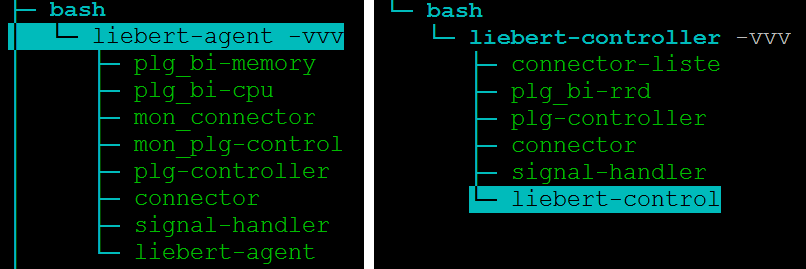
\includegraphics[width=\textwidth]{liebert-threads.png}
                \caption{\textsc{Liebert}'s thread list in \textit{htop}}
                \label{fig:thread-list}
            \end{figure}
        
        \subsubsection{Watchdog}
            With many running threads comes the issue of synchronization and thread management. To assist in this, a \textit{Watchdog} utility has been developed that is used for thread monitoring and synchronization. Currently, it's most important use case is to synchronize threads on application exit. When the user initiates a shutdown, a \textit{shutdown message} (read more in \autoref{sec:message-queue}) is sent to important threads that potentially need to do finalization before exiting. After the shutdown messages are sent, \textit{Watchdog} is used to wait for these threads to quit (handling all error scenarios gracefully), and the application exits, killing all non-important threads immediately.
        
        \subsubsection{Drawbacks}
            Unfortunately, this method has brought in some unforeseen drawbacks. Even though maximum care has been taken during development to reduce memory usage to a minimum, utilizing the multi-thread model has rendered most of these efforts rather meaningless. This is caused by the operating system allocating separate stack space for each thread. The specific initial size of this allocation varies across operating systems, and as such the application's memory consumption cannot be safely predicted. On Linux, \textit{Rust} provides an undocumented way of modifying the initial stack size as seen in  \autoref{fig:code-stack-memory-set}.
            
            \begin{figure}[!htb]
                \centering
                \begin{BVerbatim}
devel:~$ RUST_MIN_STACK=49000 ./target/release/liebert-controller
                \end{BVerbatim}
                \caption{Adjusting initial stack size by using an environment variable}
                \label{fig:code-stack-memory-set}
            \end{figure}
            
            This however seems to have some sort of a lower limit, as even though the lowest we managed to get using this approach was \textbf{4.9kB} (the option appears to be in bytes; lower values started throwing segmentation faults during application initialization), the resulting threads always allocated a minimum of \textbf{2MB}. We can look up detailed memory consumption information using the \textit{pmap} utility, invoked with the \textit{-x} flag for extended details.
            
            \begin{figure}[!htb]
                \centering
                \begin{BVerbatim}
devel:~$ ./target/release/liebert-controller
devel:~$ pmap -x <pid> | sort -nk 2 | tail -n 5
00007f6b161be000    2048       0       0 ----- libc-2.21.so
00007f6b13a00000    4096      48      48 rw---   [ anon ]
00007f6b14c00000    4096      24      24 rw---   [ anon ]
00007f6b15600000    6144     344     344 rw---   [ anon ]
00007f6b14200000    8192     116     116 rw---   [ anon ]
                \end{BVerbatim}
                \caption{Controller memory footprint using stock stack size}
                \label{fig:code-stack-memory-stock}
            \end{figure}
            
            Inspecting \autoref{fig:code-stack-memory-stock}, we see that our threads utilize \textbf{8MB}, \textbf{6MB}, \textbf{4MB} and \textbf{2MB} (not included in the figure). The largest thread is most probably the main thread, as \textit{Rust} usually allocates \textbf{8MB} for this thread on Linux, and it cannot be brought lower using the \textit{RUST\_MIN\_STACK} environment variable. The cause of the size of the rest of the threads is unknown, as they seem to randomly vary between 2, 4, and 6 megabytes. Note that you can find the full output of the \textit{pmap} utility for the default settings of \textit{liebert-controller} in \textbf{Appendix B} (\autoref{apd:pmap-controller}), and \textit{liebert-agent} in \textbf{Appendix C} (\autoref{apd:pmap-agent}).
            
            Trying to get more insight into the thread memory usage and relevance of the mysterious environment variable, we can try running the application with an exorbitant minimum stack size to determine if the environment variable in fact does something or not (\autoref{fig:code-stack-memory-custom}).
            
            \begin{figure}[!htb]
                \centering
                \begin{BVerbatim}
devel:~$ RUST_MIN_STACK=12000000 ./target/release/liebert-controller
devel:~$ pmap -x <pid> | sort -nk 2 | tail -n 5
00007fb852fab000   11716      12      12 rw---   [ anon ]
00007fb853b1d000   11716      12      12 rw---   [ anon ]
00007fb85208f000   13764      28      28 rw---   [ anon ]
00007fb85468f000   15812     348     348 rw---   [ anon ]
00007fb850e8f000   17860     116     116 rw---   [ anon ]
                \end{BVerbatim}
                \caption{Controller memory footprint using custom stack size}
                \label{fig:code-stack-memory-custom}
            \end{figure}
            
            We can see a curious phenomenon happening in \autoref{fig:code-stack-memory-custom}. Even though the stock 8MB was more than enough for the main thread, once we set the minimum stack size to 12MB, it ended up allocating more than \textbf{17MB}. The reason for this is unknown, and a closer look on the inner working of threads in \textit{Rust} (or in general) would be required, however is out of scope of this project. The same situation occurs with some of the other threads as well, as we can see that previously they consumed 6MB or less, now they take up up to almost \textbf{16MB}. We can probably assume that the threads that allocated ~12MB are the same ones that previously allocated 2MB (no thread ever allocated less regardless of the stack size setting).

            
    
    \subsection{Data flow}\label{sec:data-flow}
        The modular nature of the application allows for a quite peculiar data flow. This is a direct consequence of the multi-threading model described in the previous section, as the data needs to be moved safely and efficiently between different threads. This is done using a \textit{message queue} (read more in the next section). The application contains the following data-related modules:
        
        \textbf{Core} - Application's main event loop. Data passing from one end of the application uses it to get routed to the other end. Additionally used for system events such as initiating a shutdown.
        
        \textbf{Connector} - Used for connecting to a controller and receiving commands (\textit{Agent}), or for spawning read / write threads for incoming connections (\textit{Controller})).
        
        \textbf{Plugin Controller} - Handles available gatherer or storage backends. Forwards data received from \textbf{Core} to appropriate storage backends (\textit{Controller}.
        
        \textbf{Signal Handler} - Special purpose thread monitoring interrupt signals. Sends a \textit{shutdown message} to \textbf{Core} if an interrupt signal is detected (\textit{SIGINT} or \textit{SIGTERM}).
        
        \textbf{Plugin Threads} - Individual threads running gatherer or storage backends. Send gathered data directly to \textbf{Core} (\textit{Agent}), or receive data from a \textbf{Plugin Controller} (\textit{Controller)}.
        
        \textbf{Connection Threads} - Threads spawned for communicating with connected \textit{Agents}.
    
        \begin{figure}[!htb]
            \centering
            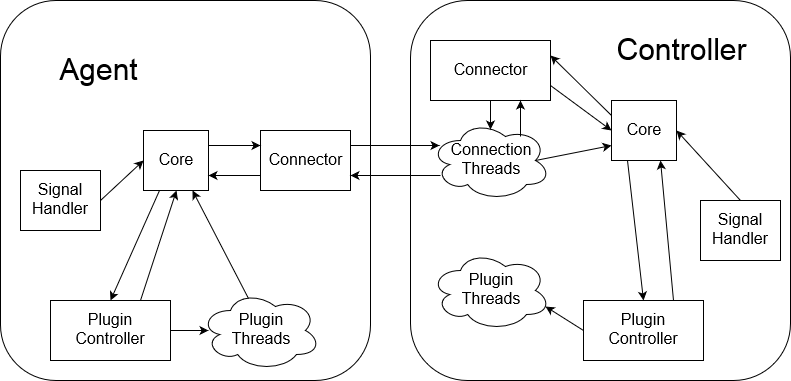
\includegraphics[width=\textwidth]{diagram-dataflow.png}
            \caption{Data flow within both applications}
            \label{fig:diagram-dataflow}
        \end{figure}
    
    \subsection{Message queue}\label{sec:message-queue}
        Due to the heavy threading within both applications, a safe and efficient way of passing data between threads had to be used. This is accomplished by using the \textit{Rust} primitive known as \textbf{channels}. These provide a memory-safe way of exchanging data between threads. Creating a channel results in two items: a \textit{sender} and a \textit{receiver}. By using \textit{Rust's} memory safety traits, channels are always restricted to a single \textit{receiver} and an unlimited number of \textit{senders}. The \textit{senders} provide a quasi-atomic means of enqueueing any sort of structure or value that can later be sequentially read through the relevant \textit{receiver}. The \textsc{Liebert} standardized structure for exchanging data between threads is a \textit{Message}, which can be seen in \autoref{fig:code-message-agent}. Note that the specific message implementation varies slightly between the two applications due to optimization reasons (more details about this are in \autoref{sec:shared-code}).
    
    \subsection{Built-in collectors}
        As stated in the requirements, the application must come with a set of built-in metric gatherers. This is a cornerstone of the project because the application only guarantees maximum performance with the built-in gatherers, as opposed to external plugins. The version of the application at the time of writing this report only contains the essential gatherers: CPU and memory.
    
        \subsubsection{CPU}
            There are multiple ways of retrieving CPU statistics under Linux. Many of them have been considered before implementation of this module, including \textit{mpstat}, \textit{/proc/stat}, \textit{top} or the average load data in \textit{uptime}. Due to the high-performance nature of this project, an approach using \textit{/proc/stat} has been chosen. Most, if not all, of the other choices required spawning an external process which incurs an unpredictable performance and memory overhead, as well as no guarantee of accurate results. The final solution reads raw CPU stats, or so called \textit{jiffies} \footnote{Jiffies are the amount of time a CPU spent on a task, they typically represent hundredths of a second}, from the system's \textit{/proc/stat} file and calculates the CPU usage accordingly. This, apart from being fast, has the added benefit of being able to calculate the exact CPU usage between any two moments in time.
        
        \subsubsection{Memory}
            The memory gatherer utilizes the standard and simple \textit{/proc/mem} file which provides detailed break-down of current memory state. More specifically, it extracts the \textbf{total}, \textbf{free}, \textbf{buffers}, and \textbf{cache} fields. These are the most important and well-known memory metrics and can be used to gain valuable insight into the current state of the system's memory.
        
    \subsection{Configurability}\label{sec:config}
        As per the original requirement, \textsc{Liebert} has been written with configurability in mind. Many parts of the application have ties to the in-memory configuration already, often even for settings that aren't available to be configured (yet). The in-memory configuration is built at the application's initialization inception, in fact it is only preceded by the creation of the main event loop send / receive channel. The configuration construction consists of two distinct but both very important steps.
        
        First, a configuration structure gets created from the command line arguments passed to the application. This is accomplished by using the handy \textbf{clap} library, which immensly eases the creation and management of command line arguments. The arguments get processed by \textbf{clap}, and get transferred into a generic configuration key-value structure. At the time of writing this report, only the \textit{-v} and \textit{-c} flags are available. These are used to specify the desired logging verbosity level, and the location of the relevant configuration file. They are both so-called \textit{global} configuration options, as they are included in both applications using shared code. Note that applications don't currently have any individual command line options, however the infrastructure for them is ready. All that needs to be done is specify the options and they will automatically work in the same way as the currently available \textit{global} ones. It is also worth mentioning that the options default to a sensible preset value if they are omitted from the command line, therefore both applications can be safely run without either the \textit{-c} or \textit{-v} flag. An automatically generated help menu is available by using the \textit{-h} or \textit{--help} switch, an example can be seen in \autoref{fig:agent-help}.
        
        \begin{figure}[!htb]
            \centering
            \begin{BVerbatim}
Liebert Agent 0.2.0
(c) Martin Kukura
Endpoint application of the Liebert monitoring platform.

USAGE:
liebert-agent [FLAGS] [OPTIONS]
FLAGS:
-h, --help       Prints help information
-V, --version    Prints version information
-v, --verbose    Verbose output
OPTIONS:
-c, --conf <conf>    Path to the configuration file
            \end{BVerbatim}
            \caption{Help output printed by the \textit{Agent} application}
            \label{fig:agent-help}
        \end{figure}
        
        After the command line argument parsing is finished, a second configuration structure is created by parsing the specified configuration file. The configuration file format is \textbf{TOML}\footnote{Tom's Obvious, Minimal Language}. This unusual format has been chosen because its parsing library is the most popular and mature configuration parsing library for \textit{Rust}, and because it is de facto an updated version of the well known \textit{ini} format mostly used in older versions of Windows. During the parsing, all directives are checked against an existing list of key-value pairs - if a defiend directive is missing from the configuration file, it is replaced by the default value specified; if the configuration file contains a directive that wasn't defined, it is simply ignored. This hardcoded directive checking was a conscious design decision in hope of reducing configuration errors - if an option is missing, the user is warned and a default is used instead of crashing the application. An example of the application warning the user of missing configuration options can be found in \autoref{fig:agent-init-warning}.
        
        Once both parsing steps are finished, the configuration is merged into a single structure. It is very important that the command line argument options are merged on top of the configuration file ones, as specifying arguments on the command line is generally regarded as the most desired setting, and should therefore overwrite any other same settings. After a careful merge, the resulting structure is enclosed in a special thread-safe "object". A reference to this configuration structure is then cloned everywhere throughout the application, allowing every thread to safely access any configuration option at will, without needing to wastefully copy the entire contents of the configuration.The only moment where parts of the data are copied from within the configuration structure is when they are requested, as they must be available to the calling thread for an indeterminate amount of time and holding a mutex lock for the entire duration would negatively affect the performance of any other threads that need access to the configuration. The specific \textit{Rust} structure used for the configuration can be found in \textbf{Appendix E} (\autoref{apd:config}).
        
        \begin{figure}[!htb]
            \centering
            \begin{BVerbatim}
devel:~$ ./target/release/liebert-controller
<init>: 'builtin.rrd.enabled' not found in configuration file,
    using default value of 'true'
<init>: 'builtin.rrd.data' not found in configuration file,
    using default value of '/tmp'
<init>: 'controller.secret' not found in configuration file,
    using default value of 'd34db33f'
<init>: 'builtin.rrd.binary' not found in configuration file,
    using default value of '/bin/rrdtool'
<init>: Plugin 'plugin-one' is enabled. [/tmp/plugin]
            \end{BVerbatim}
            \caption{Incomplete configuration warnings emitted by \textit{Controller}}
            \label{fig:agent-init-warning}
        \end{figure}
        
    
    \subsection{Noteworthy issues}\label{sec:notable-issues}
        What follows is a short list detailing the most interesting problems encountered, and the attempts at resolving them.
    
        \subsubsection{String optimization attempt}
             There are 2 types of strings in rust: a heap allocated dynamic \textit{String} and a stack allocated \textit{string slice} or \textit{\&str}. Currently, most of the strings in the application are the dynamic \textit{String} version. Even worse, whenever they are passed around they will usually be cloned, instead of being passed as a \textit{string slice reference}. An attempt has been made to convert some of this redundant \textit{String} cloning into the non-dynamic 0-overhead \textit{string slice} version, unfortunately, at least for now, this attempt has been unsuccessful. The main factor in this failure was the concurrent nature of the application. High percentage of the strings found withing the application originate from within a configuration hashmap-like structure. Due to the structure being shared between many threads, it is being hidden behind a mutex and other Rust specific concurrency tools, rendering the data inaccessible after the initial call site. Being unable to access the original string after the retrieval function without cloning prevents the usage of \textit{string slices} that could refer to the already-existing \textit{String} in the configuration structure.
        
        \subsubsection{Shared code}\label{sec:shared-code}
            A decent amount of time has been spent on optimizing the file structure of the project, and refactoring the code to reflect the changes introduced. Originally, most of the code has been built with the idea that it will be shared between both the \textit{Agent} and the \textit{Controller} application. With the introduction of the \textit{Controller} application, it has however been discovered that many of these shared structures and functions need to slightly differ between the applications, and therefore both cannot utilize the same underlying code. The problematic portions have been refactored into separate \textit{Rust modules} for each binary, reducing unnecessary bloat compiled into each application.
             
            To illustrate the problem, let's take a look at a core structure called \textit{Message}. \textit{Messages} are used extensively throughout both applications to communicate between threads, of which there are plenty (\autoref{sec:threads}). The original \textit{Message} used in \textit{Agent} can be seen in \autoref{fig:code-message-agent}.
            
            \begin{figure}[!htb]
                \centering
                \begin{BVerbatim}
pub enum Message{
    Data(String, i64, String),
    Format(String, Vec<::types::MetricFormat>),
    Shutdown(String),
    Fatal(String)
}
                \end{BVerbatim}
                \caption{\textit{Message} structure used in \textit{Agent}}
                \label{fig:code-message-agent}
            \end{figure}
            
            While implementing the \textit{Controller}, it has been found that this enum is not suitable, and therefore was to what is pictured in \autoref{fig:code-message-controller}.
            
            Note that both enums are incredibly similar, however to accommodate the internal working of the controller, a different signature was required for some of the options. Additionally, the \textit{Agent} utilizes one more option, which, due to \textit{Rust's} exhaustive pattern matching requirements, would require the \textit{Controller} code to check for its possibility in every operation involving the \textit{Message} enum.
            
            \begin{figure}[!htb]
                \centering
                \begin{BVerbatim}
pub enum Message {
    Data(String, String, u32, Vec<i64>),
    Format(String, String, Vec<::types::MetricFormat>),
    Shutdown(String)
}
                \end{BVerbatim}
                \caption{\textit{Message} structure used in \textit{Controller}}
                \label{fig:code-message-controller}
            \end{figure}
            
            Wherever possible, code has been refactored to suit both applications and is accessible from a shared module. Additionally some functions previously created for \textit{Agent} were changed to allow them to be shared with the \textit{Controller}, such as the signal handler responsible for detecting \textit{SIGTERM} and \textit{SIGINT} signals. Previously it contained hardcoded behaviour upon detection, whereas it has been changed to accept a closure, allowing each application to provide custom handling logic.
        
        \subsubsection{CPU usage reduction}
             The nature of the application suggests that much of the time it will be running will be spent idle. While idle, it should ideally consume the least amount of CPU time possible. Most application idling has been done using a while loop that checks the current time against the desired wait time. Originally, to conserve CPU time, a \textit{thread::yield\_now()} function was called within the loop, which gives up the program's allocated timeslice back to the OS scheduler. As it turns out, this does not prevent 100\% CPU usage, instead it consumes all the CPU time that is available (which means if other processes need 50\% of the CPU, our application would consume the remaining 50\%). To ease the CPU load, the function has been changed to \textit{thread::sleep()}. The current function can be seen in \autoref{fig:wait-function}:
             
             \begin{figure}[!htb]
                \centering
                \begin{BVerbatim}
pub fn wait_exec_result
(wait: Duration, exec: &Fn() -> bool) -> Result<(), ()> {
    let start = time::Instant::now();

    while start.elapsed() < wait{
        if exec(){ return Ok(()); }
        thread::sleep(time::Duration::from_millis(100));
    }
    
    Err(())
}
                \end{BVerbatim}
                \caption{Implementation of a custom thread sleep function}
                \label{fig:wait-function}
            \end{figure}
            
            Note that this does more than merely sleep for a specified amount of time (and therefore is needed instead of a simple call to \textit{thread::sleep()}) - it executes a custom function on every loop. This is used to detect when a thread received a shutdown command while sleeping. If this entire waiting function was substituted with a single call to \textit{thread::sleep()} with the desired wait time, the thread would become unresponsive until the sleep expired.

            Different approaches in regards to threading and blocking could be implemented, however are out of scope of this project. More details about these ideas can be found in \autoref{sec:future-work}.

        
        \subsubsection{Data loss on connection interruption}
             One of the project's requirements is that the \textit{Agent} instance should buffer its collected data in the event of loss of \textit{Controller} connection. Rust's I/O, including all networking, is unfortunately \textit{blocking}, meaning it cannot be easily set up to respond to incoming data using event handling, and any such approach needs to be coded manually from scracth. Due to this, \textit{Agent} spawns 3 threads for its networking functionality: a reader thread to send data over the wire, a writer thread to receive and parse incoming data, and a controlling thread to handle message direction and thread synchronization. Due to this architecture, whenever the remote end disconnects, the reader thread exits immediately. In such event, the writer thread needs to be closed manually, the connection re-established and both I/O threads restarted. To persist the buffered data, a proper concurrent safe structure had to be chosen. This has been determined to be the \textit{Sender / Receiver channel}, widely used for message passing between threads. It has been chosen over a more simple structure such as an array because it can handle a single reader and multiple writers in parallel, without the need for locking. To enable the reader end to be shared between multiple threads (in the event of the writer thread restarting), the following has been done:
             
             \begin{figure}[!htb]
                \centering
                \begin{BVerbatim}
type ConnectorMessageReceiver = Receiver<Message>;
type ConnectorMutexedReceiver = Arc<Mutex<ConnectorMessageReceiver>>;
                \end{BVerbatim}
                \caption{Encapsulation of a \textit{Receiver} for sharing between threads}
                \label{fig:receiver-mutex}
            \end{figure}

            This allows the reading end of the channel to be shared across threads (unavailable otherwise due to Rust's memory safety guarantees). Whenever a new writer thread gets created, it obtains a mutex lock to the receiving end of the channel and can begin processing. Due to the RAII implementation of Rust's mutex locks, when this thread exits (error or manual shutdown), it releases the lock automatically, allowing a newly spawned thread to start receiving on the same channel.
